\documentclass[10pt,a4paper]{article}
\usepackage[margin=1.8cm]{geometry}
\usepackage[T1]{fontenc}
\usepackage[utf8]{inputenc}
\usepackage[italian]{babel}
\usepackage{amsmath,booktabs,graphicx,hyperref,array}
\title{Verifiche numeriche Allen--Cahn con bordo dinamico e funzionale WED}
\author{Rapporto operativo basato sulla proposta per la sezione numerica}
\date{22 ottobre 2026}
\begin{document}
\maketitle

\section*{Sintesi}
Ho applicato i test raccomandati alla parte parabolica del modello. Ho aggiunto il parametro positivo \texttt{surfacebeta} alla legge Allen--Cahn: moltiplica reazione e derivata della reazione soltanto sugli elementi lineari di bordo; nel bulk resta la legge esistente. Lo stesso coefficiente è stato aggiunto al prototipo WED Python. Il valore predefinito è 1, quindi gli input precedenti mantengono la stessa equazione.

La diagnosi ha trovato due problemi distinti. Nel solver, `line1ht` usava un punto di Gauss, insufficiente per capacità e reazione Allen--Cahn: il default è stato portato a tre punti. Nel postprocessing Python, invece, la derivata lineare lungo un bordo di lunghezza $L$ era calcolata come $[-1/2,1/2]/L$ anziché $[-1,1]/L$; ciò sottostimava di un fattore quattro la rigidezza tangenziale e l'energia di gradiente superficiale. Ho corretto il gradiente negli script energetici, WED e di studio di $\beta$. Gli input Allen--Cahn usano inoltre `nip 9` sui quadrilateri per integrare esattamente la reazione cubica Q1. Il residuo energetico ora diminuisce regolarmente al raffinarsi del passo temporale.

\section{Equazioni, implementazione e portata}
Il sistema studiato è
\[
 u_t-\Delta u+u^3-u=0\quad\hbox{in }\Omega,\qquad
 u_{\Gamma,t}-\Delta_\Gamma u_\Gamma+\beta(u_\Gamma^3-u_\Gamma)=-\partial_nu\quad\hbox{su }\Gamma,
 \qquad u_\Gamma=u|_\Gamma.
\]
L'energia corrispondente usa $F(u)=\frac14(u^2-1)^2$ nel bulk e $G(u_\Gamma)=\frac{\beta}{4}(u_\Gamma^2-1)^2$ sul bordo. Il coefficiente compare sulla sorgente interna e sulla sua tangente degli elementi `line1ht`; sui quadrilateri o triangoli del bulk il suo effetto è nullo. Anche la sorgente MMS di bordo include la stessa dipendenza da $\beta$.

Il minimizzatore WED resta un programma Python di ricerca separato, che legge la mesh da un input OOFEM, assembla la formulazione FEM globale nel tempo, usa Newton sparso smorzato e salva la traiettoria VTK. Non è registrato né eseguito dall'eseguibile C++ OOFEM. I test WED verificano quel backend, non un'integrazione nativa nel solver OOFEM. I casi qui eseguiti sono 2D; il sistema a onde e il benchmark triangolare P1 proposto non sono stati implementati in questo passaggio.

Il funzionale discreto implementato è la versione troncata e riscalata in $s=t/\varepsilon$:
\[
J_\varepsilon(u)=\int_0^{S_{\max}} e^{-s}\left[\frac12\|u_s\|^2_{L^2(\Omega)\oplus L^2(\Gamma)}
 +\varepsilon\left(\frac12\|\nabla u\|^2_{L^2(\Omega)}+\frac12\|\nabla_\Gamma u_\Gamma\|^2_{L^2(\Gamma)}
 +\int_\Omega F(u)+\int_\Gamma G(u_\Gamma)\right)\right]ds,
\]
con $u(0)=u_0$, elementi lineari nel tempo, quadratura di Gauss e valore terminale libero. Il gradiente e l'Hessiana sono verificati con differenze finite direzionali. Un controllo aggiuntivo confronta $S_{\max}=6,12,18$ a $\varepsilon=0.05$, con $\Delta s=0.1$, sulla finestra fisica comune $[0,0.1]$. Rispetto a $S_{\max}=18$, le differenze RMS spazio-tempo sono $3.67\,10^{-5}$ per $S_{\max}=6$ e $1.56\,10^{-7}$ per $S_{\max}=12$; le massime differenze nodali sono rispettivamente $3.02\,10^{-4}$ e $1.13\,10^{-6}$. Questa è una misura del troncamento per quel caso, non una stima uniforme.

\paragraph{Parametri dei benchmark.} Per il test non uniforme di limite WED il dominio è $[0,2]\times[0,1]$ e $u_0(x,y)=0.2+0.1[\cos(\pi x/2)\cos(\pi y)+0.25\sin(\pi x/2)\sin(\pi y)]$, con $\beta=1$ e sorgente MMS disattivata. La tabella esplicita i parametri di riproduzione; il riferimento diretto è sempre il solver C++ OOFEM, mentre il campo WED è prodotto dal minimizzatore Python.
\begin{center}\small
\begin{tabular}{p{2.5cm}p{3.0cm}p{3.8cm}p{4.2cm}}
\toprule
studio & dominio, dati e mesh & parametri WED & riferimento/criterio\\
\midrule
limite $\varepsilon$ & rettangolo $2\times1$, $u_0$ sopra, mesh $8\times4$, $\beta=1$ & $S_{\max}=12$, $\Delta s=0.1$, tol $2\,10^{-5}$; inoltre $\Delta t=0.005$ fisso & OOFEM diretto $\Delta t=0.001$, errore spazio-tempo su $[0,0.1]$\\
orizzonte & stessi dati e mesh & $\varepsilon=0.05$, $\Delta s=0.1$, tol $2\,10^{-5}$, $S_{\max}=6,12,18$ & traiettoria $S_{\max}=18$ su $[0,0.1]$\\
convergenza mesh & stesso dominio e $u_0$, mesh $8\times4$, $16\times8$, $32\times16$ & $\varepsilon=0.05$, $S_{\max}=12$; base $\Delta s=0.1$, tol $2\,10^{-5}$; robustezza $\Delta s=0.05$, tol $2\,10^{-6}$ & soluzione WED fine come riferimento numerico, errore su $[0,0.1]$\\
MMS diretto & stesso rettangolo, mesh Q1 raffinate & non usa WED; OOFEM $T=0.02$, $\Delta t=5\,10^{-4}$, $\beta=1$ o 2 & soluzione fabbricata esatta, RMS nodale\\
\bottomrule
\end{tabular}
\end{center}

\section{Test A: limite $\varepsilon\to0$ dei minimizzatori WED}
Il test principale usa il campo iniziale non uniforme definito sopra sul rettangolo $[0,2]\times[0,1]$, mesh $8\times4$ quadrilateri e gli stessi nodi per OOFEM e WED. La sorgente MMS è spenta: entrambi risolvono il problema non forzato. Il riferimento OOFEM usa $\Delta t=10^{-3}$. Si confrontano norme $L^2$ FEM bulk e bordo integrate su $t\in[0,0.1]$. Nei quattro casi vario solo $\varepsilon\in\{0.1,0.05,0.025,0.0125\}$: $S_{\max}=12$, $\Delta s=0.1$, tolleranza di ottimizzazione $2\,10^{-5}$ e limite 100 iterazioni sono fissi. Ogni minimizzazione termina in 2 iterazioni e richiede circa 0.8 s.
\begin{center}
\small
\begin{tabular}{rrrrrr}
\toprule
$\varepsilon$ & $E_\Omega$ & $E_\Gamma$ & iterazioni & tempo [s] & p sperimentale\\
\midrule
0.1000 & $1.8485\,10^{-3}$ & $3.1960\,10^{-3}$ & 2 & 0.792 & --\\
0.0500 & $1.1511\,10^{-3}$ & $2.0198\,10^{-3}$ & 2 & 0.810 & 0.684/0.662\\
0.0250 & $6.8730\,10^{-4}$ & $1.1978\,10^{-3}$ & 2 & 0.779 & 0.744/0.753\\
0.0125 & $3.8735\,10^{-4}$ & $6.6759\,10^{-4}$ & 2 & 0.800 & 0.828/0.843\\
\bottomrule
\end{tabular}
\end{center}
Entrambi gli errori integrati calano al diminuire di $\varepsilon$. Le pendenze in tabella sono stime locali bulk/bordo dai punti adiacenti, non ordini teorici. Il controllo direzionale di gradiente e Hessiana è dell'ordine di $10^{-9}$. A $\varepsilon=0.05$, dimezzare $\Delta s$ da 0.1 a 0.05 (passo fisico da 0.0025 a 0.00125) cambia gli errori solo nelle ultime cifre: rispettivamente $E_\Omega=1.15128\,10^{-3}$, $E_\Gamma=2.02008\,10^{-3}$ e $E_\Omega=1.15132\,10^{-3}$, $E_\Gamma=2.02015\,10^{-3}$. Un controllo omogeneo aggiuntivo, confrontato anche con l'ODE esatta, mostra una riduzione più netta; i dati sono nel CSV.

Poiché $s=t/\varepsilon$, vale $\Delta t=\varepsilon\Delta s$: il test precedente a $\Delta s$ fisso variava anche il passo fisico. Per separare questi effetti ho ripetuto tutti e quattro i valori con $\Delta t=0.005$ fisso, scegliendo $\Delta s=0.005/\varepsilon$. La finestra di confronto con OOFEM resta $[0,0.1]$; il suo passo diretto è $0.001$. Il tempo terminale WED $\varepsilon S_{\max}$ varia con $\varepsilon$, ma resta maggiore di 0.1 anche per il valore minimo.
\begin{center}\small
\begin{tabular}{rrrrrr}
\toprule
$\varepsilon$ & $\Delta s$ & $\Delta t$ & $\varepsilon S_{\max}$ & $E_\Omega$ & $E_\Gamma$\\
\midrule
0.1000 & 0.050 & 0.005 & 1.200 & $1.8475\,10^{-3}$ & $3.1947\,10^{-3}$\\
0.0500 & 0.100 & 0.005 & 0.600 & $1.1511\,10^{-3}$ & $2.0198\,10^{-3}$\\
0.0250 & 0.200 & 0.005 & 0.300 & $6.8614\,10^{-4}$ & $1.1959\,10^{-3}$\\
0.0125 & 0.400 & 0.005 & 0.150 & $3.8299\,10^{-4}$ & $6.6022\,10^{-4}$\\
\bottomrule
\end{tabular}
\end{center}
Gli errori continuano a diminuire con $\varepsilon$ anche a passo fisico costante. Questo controllo mirato riduce la confusione dovuta al passo temporale, ma non elimina ogni errore temporale: per $\varepsilon=0.0125$ la griglia in $s$ è relativamente rada ($\Delta s=0.4$). Il dato è quindi una verifica di robustezza del trend, non una stima isolata dell'errore asintotico.

Per $\varepsilon=0.0125$ ho dimezzato ulteriormente $\Delta s$ da 0.4 a 0.2, mantenendo $S_{\max}=12$, mesh e tolleranza $2\,10^{-5}$. Con due iterazioni in entrambi i run, $E_\Omega$ passa da $3.82985\,10^{-4}$ a $3.86483\,10^{-4}$ e $E_\Gamma$ da $6.60221\,10^{-4}$ a $6.66145\,10^{-4}$: variazioni di circa 0.9\%. Le differenze spazio-tempo fra le due traiettorie sono $4.16\,10^{-6}$ nel bulk e $6.44\,10^{-6}$ sul bordo. La soluzione è quindi stabile al livello di circa 1\% per questa verifica; l'errore contro il riferimento non diminuisce monotonicamente col solo raffinamento temporale.

\begin{center}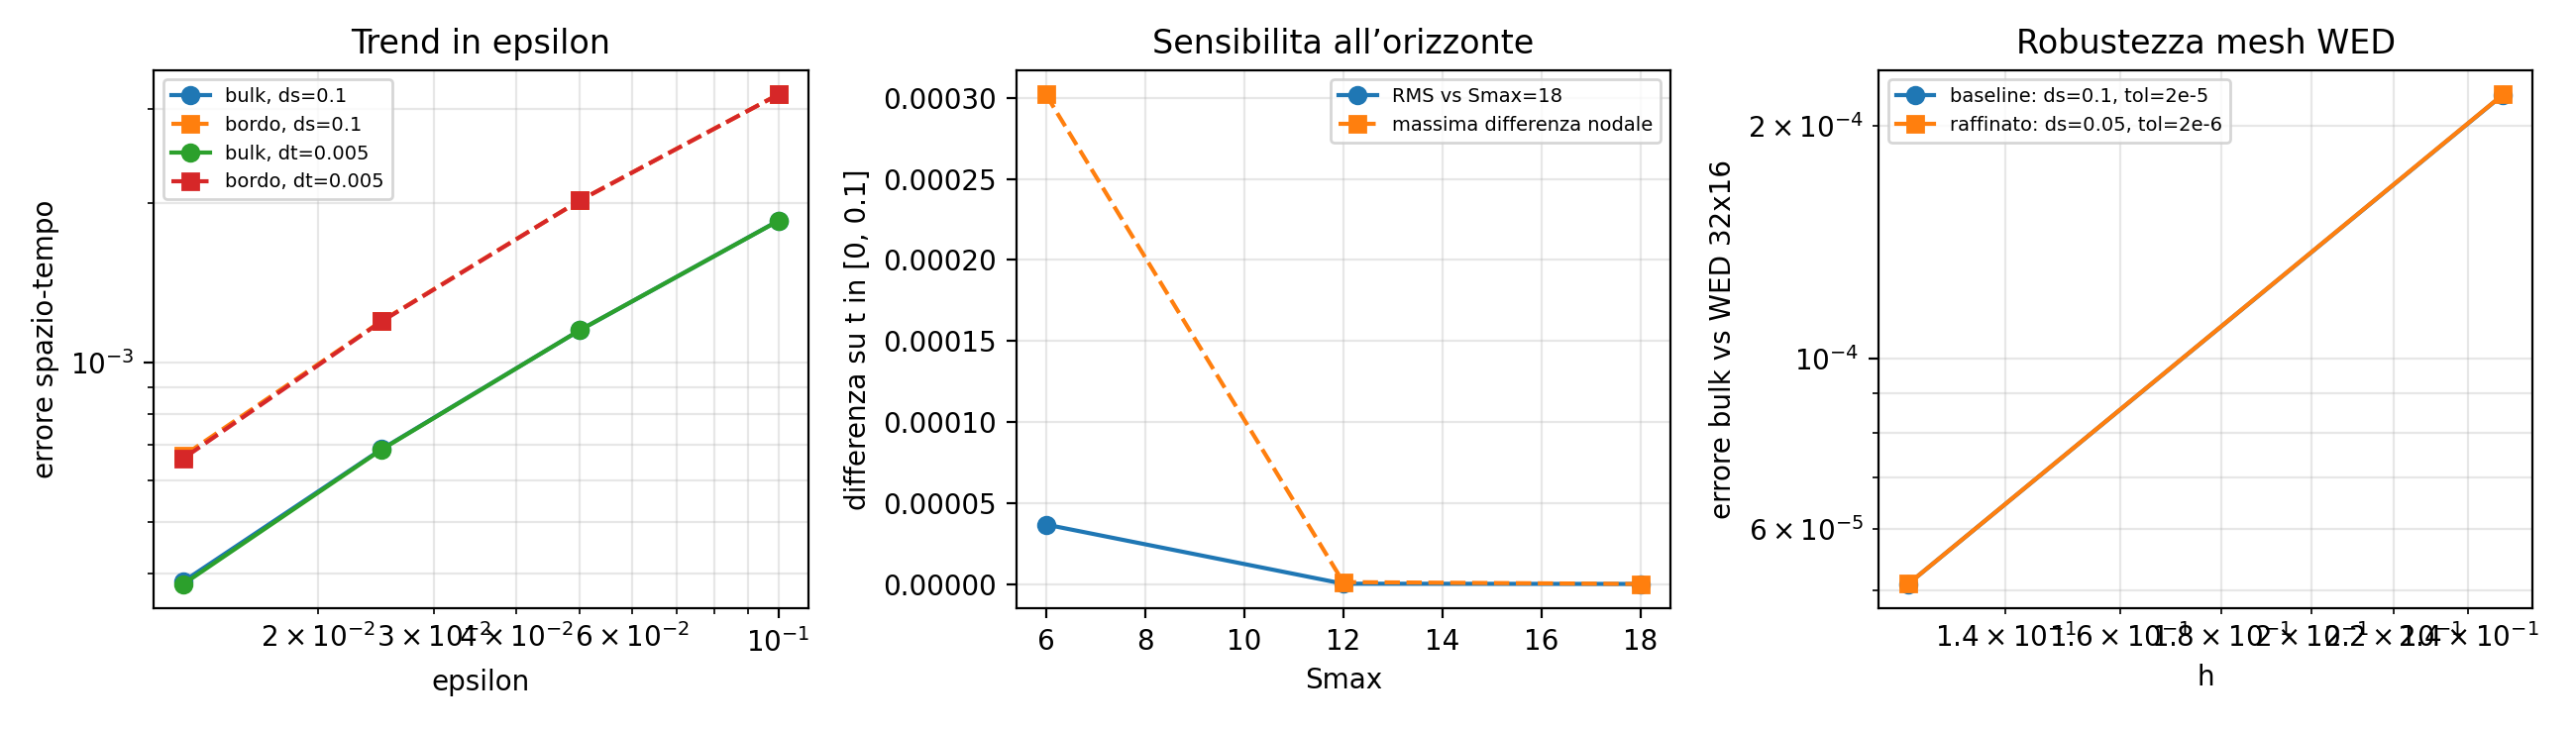
\includegraphics[width=0.99\linewidth]{wed_checklist_robustness.png}\end{center}

\begin{center}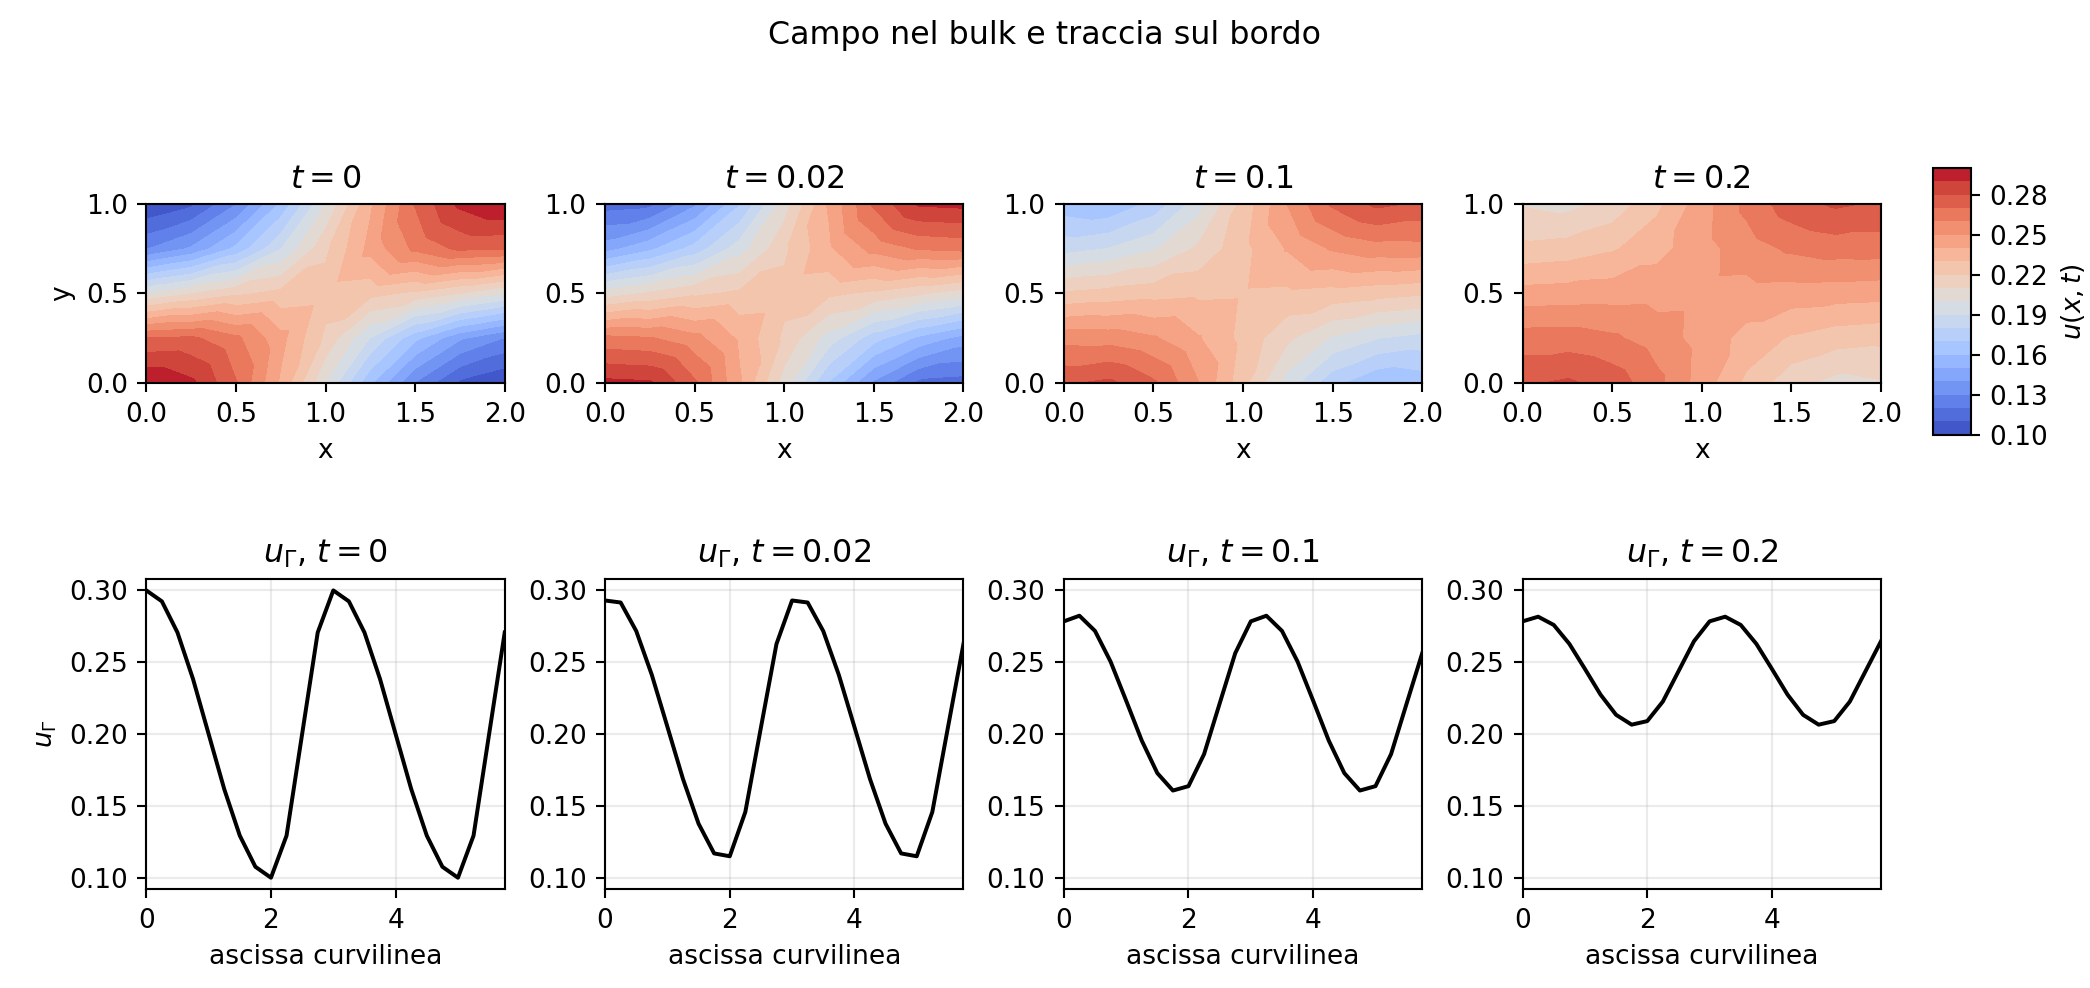
\includegraphics[width=0.90\linewidth]{field_and_boundary_snapshots.png}\end{center}
La figura mostra snapshot del campo e la sua traccia sulla frontiera a $t=0$, $0.02$, $0.1$ e $0.2$ per il benchmark non uniforme.

\begin{center}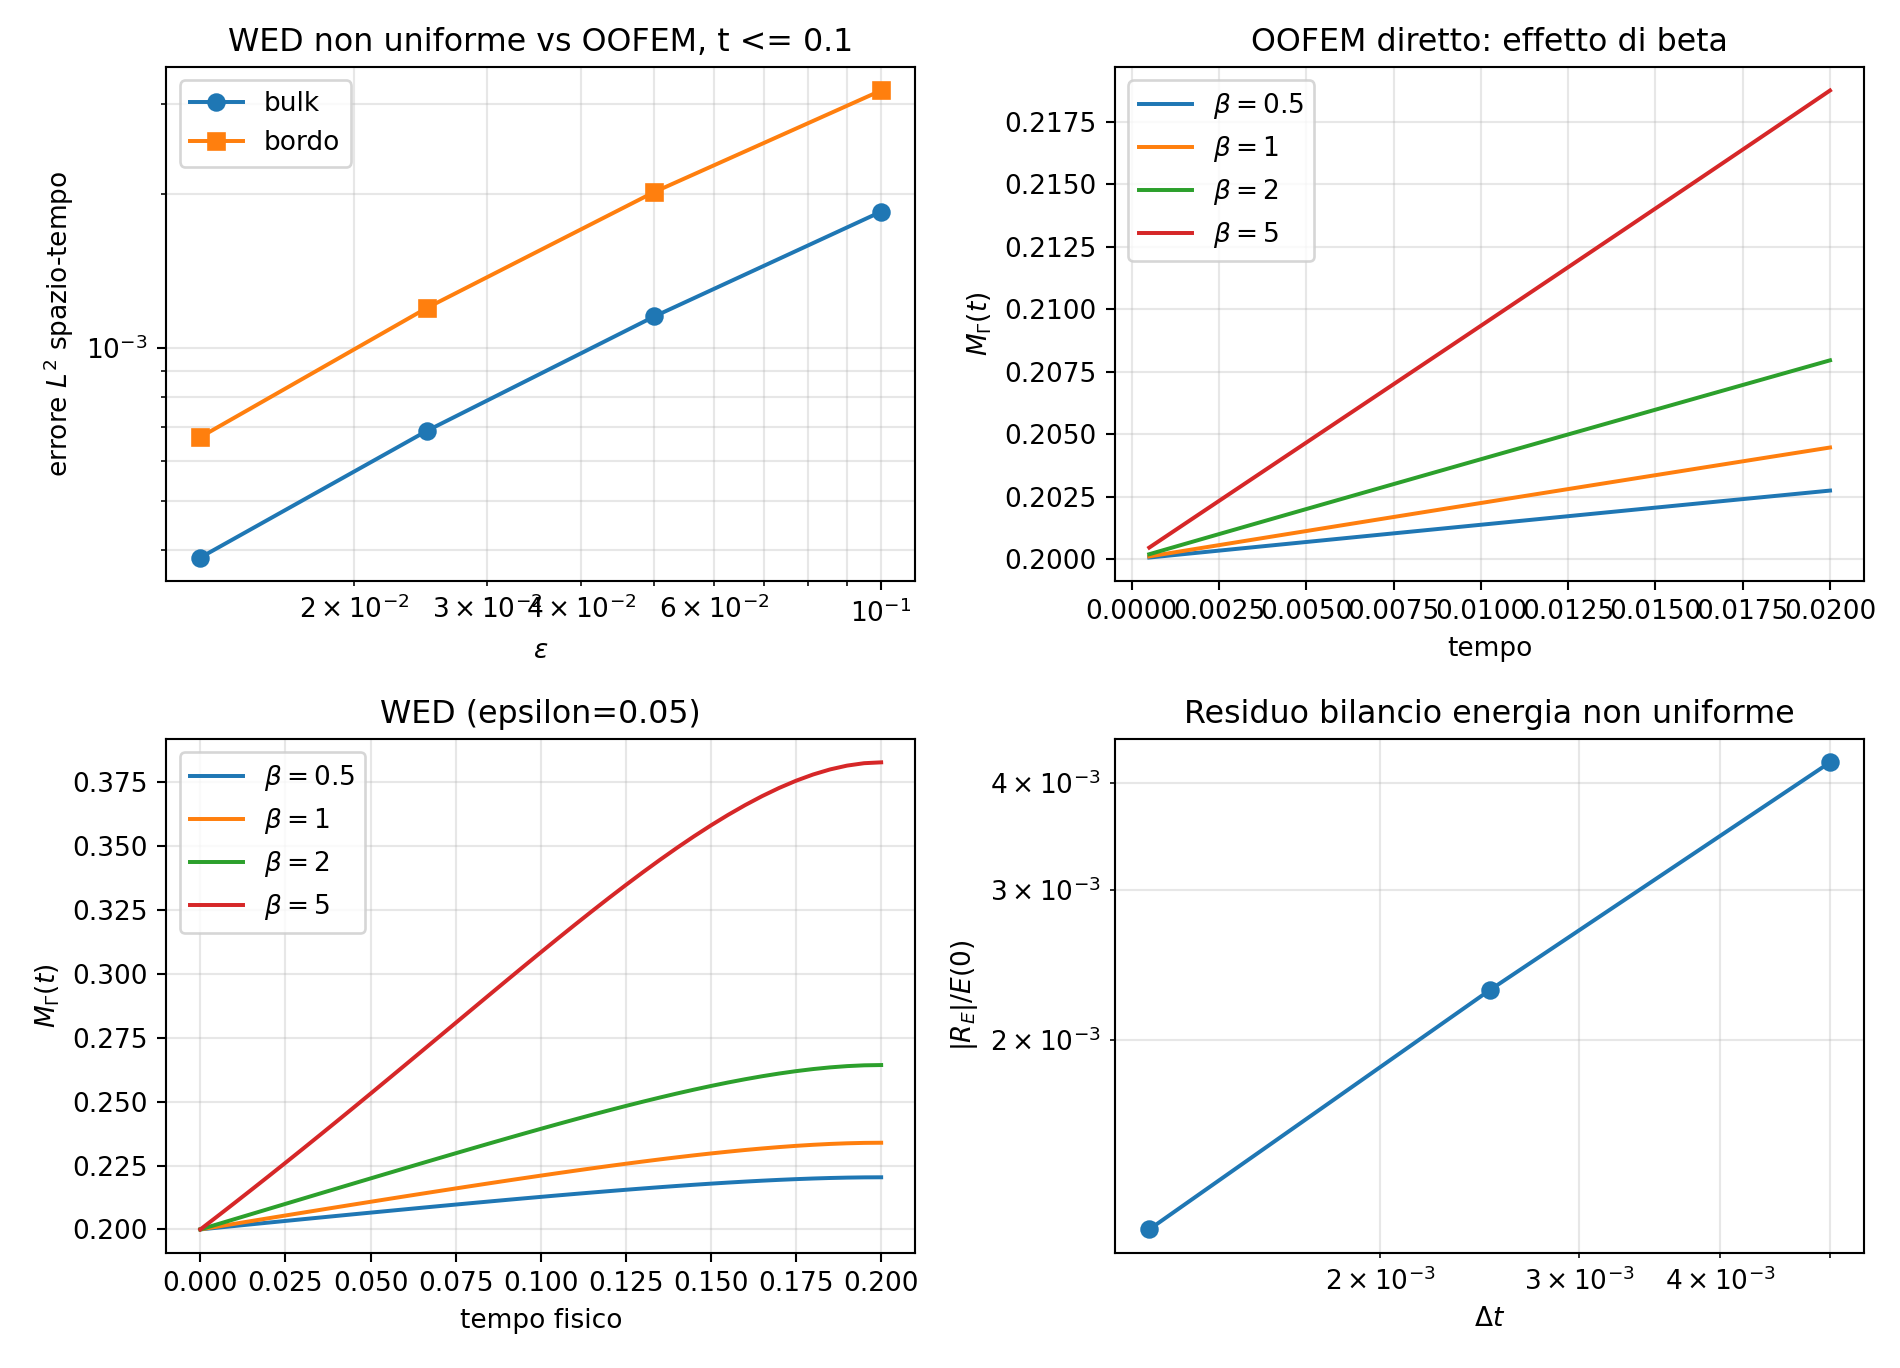
\includegraphics[width=0.96\linewidth]{recommended_tests.png}\end{center}

\section{Test B: dissipazione e residuo della legge energetica}
Per il caso non forzato su mesh $20\times20$, $T=0.5$ e $\Delta t=0.0125$, l'energia discreta totale corretta è decresciuta monotonamente nei 40 passi registrati: da 1.252362 al primo passo a 1.155833 all'ultimo.

Ho inoltre calcolato
\[
 R_E=E(T)-E(0)+D_\Omega+D_\Gamma,\qquad
 D_{\Omega,\Gamma}=\int_0^T\!\int_{\Omega,\Gamma}|u_t|^2,
\]
approssimando $u_t$ con differenze all'indietro e integrando con le matrici di massa FEM. La prima diagnosi attribuiva erroneamente lo scarto al bordo: il postprocessing usava una derivata tangenziale dimezzata, e quindi energia superficiale e rigidezza superficiale non erano coerenti con OOFEM. Dopo la correzione, su $T=0.1$ il residuo normalizzato scende da $0.423\%$ a $0.120\%$ quando $\Delta t$ passa da $5\,10^{-3}$ a $1.25\,10^{-3}$. Il residuo con segno resta negativo e tende a zero, come atteso per il controllo a passo finito con differenze all'indietro. La verifica ora supporta la coerenza energetica, pur non costituendo una dimostrazione analitica della stabilità per ogni input.

\begin{center}
\small
\begin{tabular}{rrrrrrr}
\toprule
$\Delta t$ & $E(0)$ & $E(T)$ & $D_\Omega$ & $D_\Gamma$ & $R_E$ & $|R_E|/E(0)$\\
\midrule
0.00500 & 1.284456 & 1.209120 & 0.022138 & 0.047763 & $-5.4350\,10^{-3}$ & 0.004231\\
0.00250 & 1.284456 & 1.209018 & 0.022887 & 0.049612 & $-2.9395\,10^{-3}$ & 0.002289\\
0.00125 & 1.284456 & 1.208967 & 0.023310 & 0.050636 & $-1.5420\,10^{-3}$ & 0.001201\\
\bottomrule
\end{tabular}
\end{center}
\begin{center}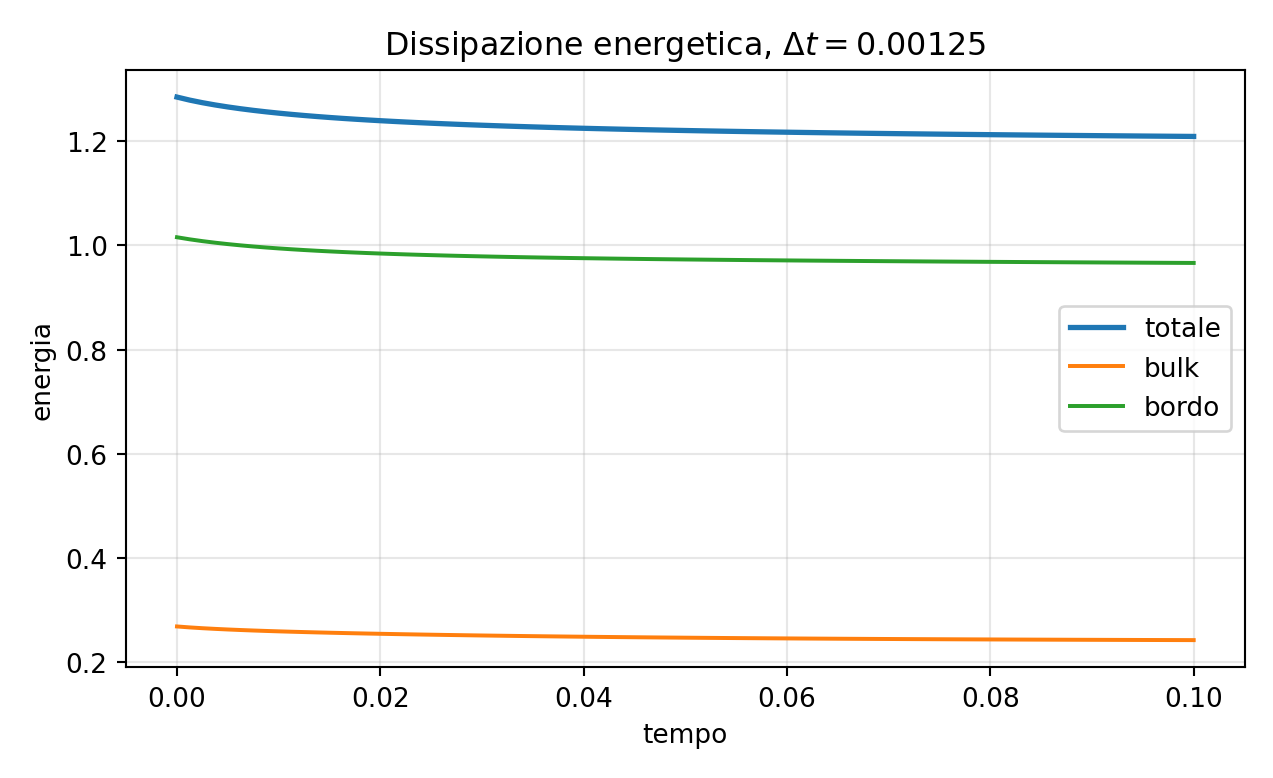
\includegraphics[width=0.78\linewidth]{energy_trajectory.png}\end{center}
Il grafico mostra i contributi bulk e superficiale e la loro somma. I contributi singoli non devono essere monotoni; qui si osserva anche la diminuzione dell'energia totale.

\section{Test C: effetto del potenziale superficiale}
Sono stati eseguiti quattro casi con $\beta\in\{0.5,1,2,5\}$ sulla stessa mesh rettangolare, stessi dati iniziali e tolleranze. Nell'evoluzione OOFEM diretta con sorgente MMS disattivata, a $T=0.02$ la media del bordo è rispettivamente 0.202747, 0.204471, 0.207959 e 0.218756. Il test MMS separato con $\beta=2$ è terminato senza errori o warning e ha RMS nodale $2.3927\,10^{-4}$ (caso $\beta=1$: $2.0634\,10^{-4}$ sulla stessa griglia e passo temporale).

Il backend WED ha inoltre risolto i quattro casi a $\varepsilon=0.05$, $S_{\max}=4$, $\Delta s=0.1$; le Newton hanno richiesto 2, 2, 2 e 3 iterazioni. La media di bordo al tempo fisico 0.2 è 0.220390, 0.233905, 0.264304 e 0.382729. Questi valori mostrano una risposta sensibile a $\beta$ per i dati scelti; i tempi finali differiscono tra il test diretto e quello WED, perciò le due serie non vanno lette come confronto punto a punto. Non si assume che la dipendenza sia monotona per ogni dato iniziale.

\begin{center}\small
\begin{tabular}{rrrrrr}
\toprule
$\beta$ & $M_\Gamma(T)$ & $E_\Gamma(T)$ & $D_\Omega$ & $D_\Gamma$ & $D_\Omega+D_\Gamma$\\
\midrule
0.5 & 0.202747 & 0.739877 & 0.005098 & 0.018408 & 0.023505\\
1 & 0.204470 & 1.423137 & 0.005238 & 0.020230 & 0.025468\\
2 & 0.207956 & 2.783037 & 0.006023 & 0.029831 & 0.035853\\
5 & 0.218748 & 6.806088 & 0.012690 & 0.109610 & 0.122300\\
\bottomrule
\end{tabular}
\end{center}
La dissipazione è integrata sul transiente diretto $T=0.02$. Non è riportato un tempo di rilassamento, perché per questi casi non è stata fissata una soglia di equilibrio.
Non è incluso un confronto con un modello privo di dinamica superficiale: occorre definire un problema al contorno alternativo che mantenga esplicito l'accoppiamento col bulk; porre semplicemente $\beta=0$ non equivale a rimuovere la dinamica di bordo.

\section{Test D: raffinamento spaziale}
Per il transiente OOFEM, la sequenza MMS quadrilatera riduce l'RMS nodale da $7.8821\,10^{-5}$ (45 nodi, $8\times4$ celle) a $1.7886\,10^{-5}$ (153 nodi) e $4.3869\,10^{-6}$ (561 nodi), con ordini osservati 2.14 e 2.03. Gli input usano `nip 9` nel bulk e tre punti sugli elementi di bordo; il caso ha $T=0.02$, $\Delta t=5\,10^{-4}$.
\begin{center}\small
\begin{tabular}{rrrrrr}
\toprule
mesh & nodi/DoF & $h$ & RMS nodale & tempo [s] & ordine $p$\\
\midrule
$8\times4$ & 45 & 0.250 & $7.8821\,10^{-5}$ & 0.398 & --\\
$16\times8$ & 153 & 0.125 & $1.7886\,10^{-5}$ & 1.380 & 2.140\\
$32\times16$ & 561 & 0.0625 & $4.3869\,10^{-6}$ & 5.374 & 2.028\\
\bottomrule
\end{tabular}
\end{center}
\begin{center}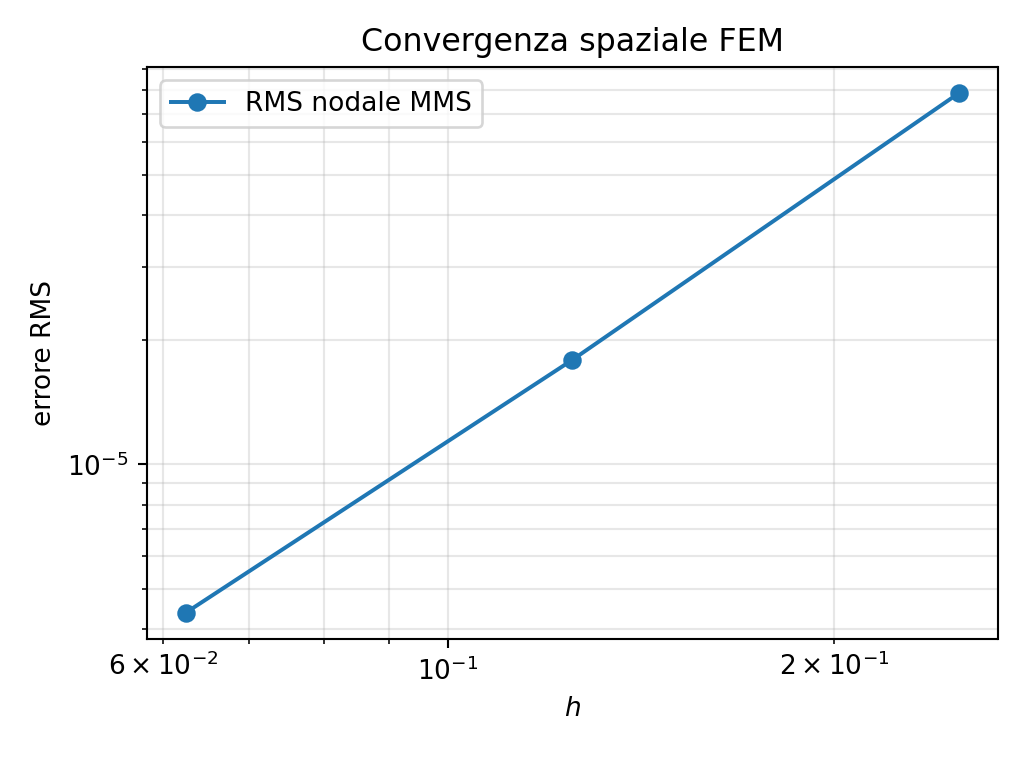
\includegraphics[width=0.52\linewidth]{spatial_convergence.png}\end{center}

Per verificare la convergenza spaziale WED, confronto le mesh coarse con WED sulla mesh fine $32\times16$, mantenendo $\varepsilon=0.05$, $S_{\max}=12$ e $\Delta s=0.1$. Riporto il confronto WED/OOFEM separatamente: contiene anche il bias dovuto a $\varepsilon>0$ e non è un test puro di raffinamento mesh.
\begin{center}
\small
\begin{tabular}{rrrrrrr}
\toprule
mesh WED & nodi & $h$ & $E_\Omega$ & $E_\Gamma$ & tempo [s] & $p_\Omega/p_\Gamma$\\
\midrule
$8\times4$ & 45 & 0.250 & $2.1961\,10^{-4}$ & $3.1175\,10^{-4}$ & 0.797 & 2.107/2.243\\
$16\times8$ & 153 & 0.125 & $5.0963\,10^{-5}$ & $6.5835\,10^{-5}$ & 2.012 & 2.107/2.243\\
$32\times16$ & 561 & 0.0625 & riferimento & riferimento & 37.735 & --\\
\bottomrule
\end{tabular}
\end{center}
Gli errori WED/WED calano di fattori 4.31 nel bulk e 4.74 sul bordo passando da $h=0.25$ a $h=0.125$, coerente con convergenza spaziale di ordine due. Il confronto separato WED/OOFEM sulla mesh coarse vale $9.17\,10^{-4}$ nel bulk e $1.63\,10^{-3}$ sul bordo: non va usato per inferire l'ordine spaziale, perché contiene il bias di $\varepsilon$.
Ho ripetuto il test sulle stesse tre mesh dimezzando $\Delta s$ a 0.05 (quindi $\Delta t=0.0025$) e stringendo la tolleranza del gradiente scalato da $2\,10^{-5}$ a $2\,10^{-6}$. Il confronto resta sulla finestra fisica $[0,0.1]$ e usa ancora la soluzione WED $32\times16$ come riferimento numerico. Gli ordini bulk/bordo stimati dalle due mesh coarse sono 2.108/2.216, contro 2.107/2.243 nel run base; le differenze sono rispettivamente 0.001 e 0.028. La tendenza spaziale di secondo ordine è quindi stabile rispetto a questo raffinamento temporale e di ottimizzazione, entro il limite del riferimento numerico fine.
\begin{center}\small
\begin{tabular}{lrrrr}
\toprule
run & $E_\Omega(8\times4)$ & $E_\Omega(16\times8)$ & $p_\Omega$ & $p_\Gamma$\\
\midrule
base: $\Delta s=0.1$, tol $2\,10^{-5}$ & $2.1961\,10^{-4}$ & $5.0963\,10^{-5}$ & 2.107 & 2.243\\
raffinato: $\Delta s=0.05$, tol $2\,10^{-6}$ & $2.1977\,10^{-4}$ & $5.0972\,10^{-5}$ & 2.108 & 2.216\\
\bottomrule
\end{tabular}
\end{center}
\begin{center}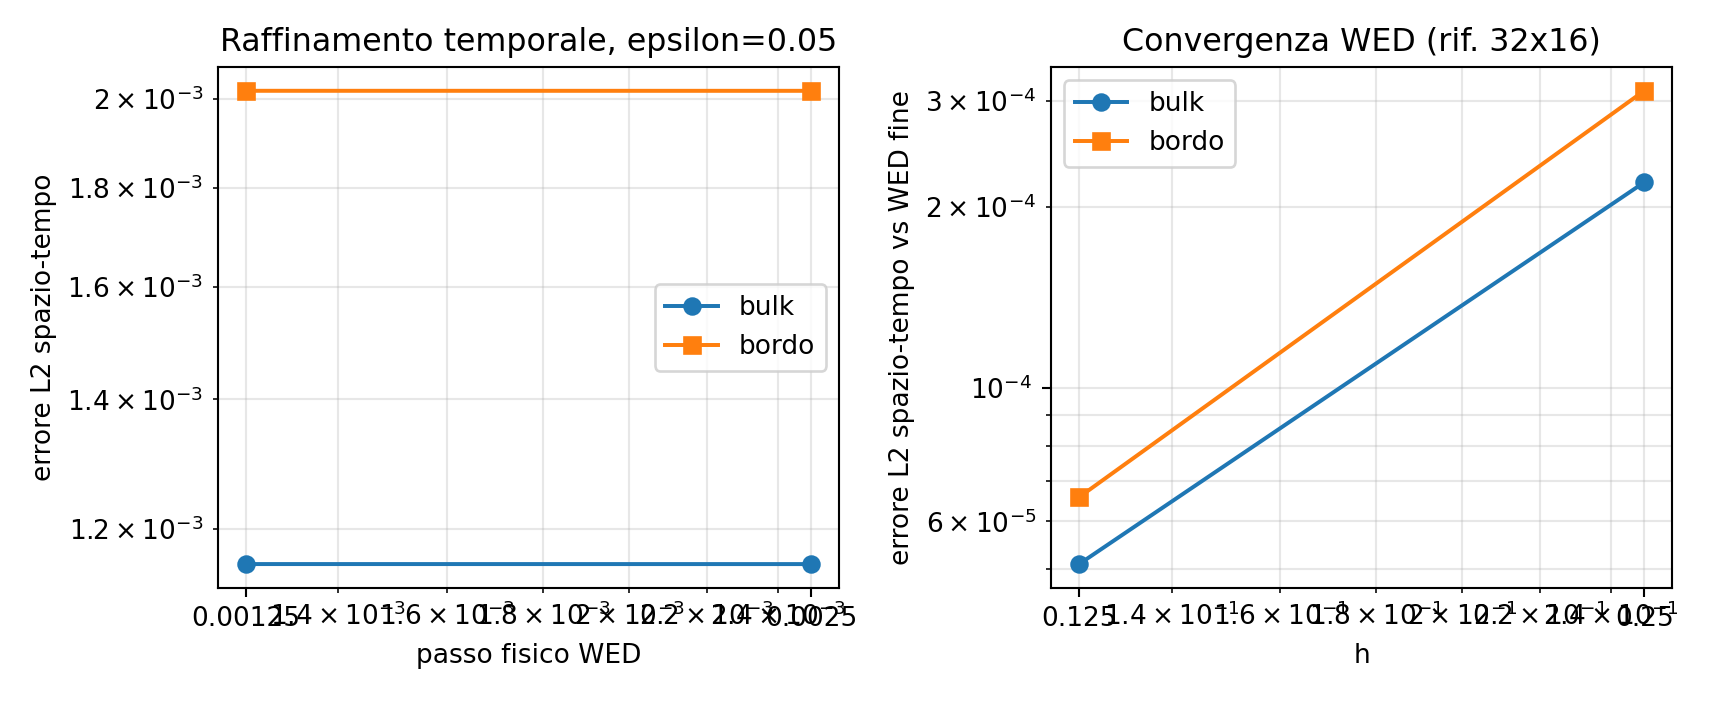
\includegraphics[width=0.80\linewidth]{wed_refinements.png}\end{center}

\section{Esito e prossimi controlli necessari}
Il parametro $\beta$ è disponibile in C++ per la reazione superficiale e in Python per il potenziale WED. Sono stati corretti il difetto di quadratura C++ su `line1ht` e il gradiente tangenziale errato nei controlli Python. Il bilancio energetico ora converge al diminuire di $\Delta t$, la convergenza spaziale WED a $\varepsilon$ fisso è osservata e la MMS diretta converge al secondo ordine. La MMS e il bilancio energetico verificano proprietà del solver diretto Allen--Cahn; i test rispetto a $\varepsilon$, all'orizzonte e alla mesh supportano invece le conclusioni numeriche sul minimizzatore WED. Lo studio $\beta$ documenta una risposta parametrica, non è da solo una verifica d'accuratezza. Questi test supportano la coerenza dell'implementazione per i casi esaminati; non costituiscono una validazione universale per ogni geometria, parametro o passo temporale.

Il paper teorico non fornisce grafici numerici o parametri di esperimenti da riprodurre: questo rapporto verifica proprietà matematiche del modello e non replica figure degli autori. La variante iperbolica a onde resta fuori ambito.

\section*{Riproducibilità}
Script, input, CSV e figure si trovano in \url{doc/stvowu_validation}. I driver principali sono i test WED omogeneo e non uniforme, il raffinamento mesh WED, lo studio beta, il bilancio energetico e il raffinamento MMS. La build usata è \url{build/debug_magneto/oofem}. Il residuo energetico usa differenze all’indietro sui campi VTU salvati; è un controllo discreto, non una stima esatta del residuo continuo.
\end{document}
